\section{Automatsko testiranje}
Jedna od bitnih aktivnost u ciklusu je automatsko testiranje softvera \cite{jenkins:2011}. Automatsko testiranje značajno unapređuje razvojni proces. Ovakvi testovi daju sigurnost da nove izmene u kodu neće pogoršati stabilnost sistema, kao i da će funkcionalnosti koje su do tada radile, nastaviti da rade. Timovi treba da ulažu u pisanje testova jer se njima podiže kvalitet proizvoda, a cena testiranja je mnogo manja u odnosu na kasnije ispravke. 

Najefikasniji pristup pisanja dobrih testova je da se testovi pišu na početku, pre pisanja samog k\^oda. Ovakva tehnika se naziva razvoj vođen testovima (eng.~{\em Test Driven Development}). U te svrhe se najčešće koriste testovi jedinica (eng.~{\em Unit tests})\cite{docs:unit}. 

U ovom poglavlju ćemo pokazati kako se u Jenkins može integrisati automatsko testiranje. Iako postoji mnogo različitih načina za testiranje softvera, držaćemo se uglavnom testova jedinica jer smatramo da je takav pristup testiranju najzastupljeniji.

\subsection{Uključivanje testova jedinica u proces}
Postoje različiti testovi jedinica za razne jezike. Najpoznatija grupa testova jedinica su \textit{x}Unit testovi, gde \textit{x} označava programski jezik (za Java programski jezik će biti JUnit, za PHP će biti PHPUnit itd.). 

\textit{x}Unit testovi kao rezultat testiranja generišu neku vrstu izveštaja u XML datoteku za koju se zna shema. To znači dve stvari. Prvo, da alati za testiranje ne moraju da budu baš iz \textit{x}Unit familije, već mogu biti bilo kakvi alati koji će svoj izveštaj generisati u XML datoteku. Drugo, da Jenkins može da parsira taj izveštaj i lepše da ga prikaže za razliku od XML datoteke.

Automatsko testiranje se izvršava kao jedna od operacija build procesa. Pošto je izlaz testiranja XML datoteka, jedino što preostaje da se uradi je da se konfiguraciji projekta postavi putanja do izlazne XML datoteke.

\subsubsection{Konfigurisanje test izveštaja i prikazivanje rezultata}
Prvo je potrebno dodati novu post-build akciju. Iz padajućeg menija treba izabrati ``Publish JUnit test result report``. Jenkins dolazi sa preinstaliranim dodatkom za JUnit test izveštaje. Ako je projekat testiran u nekom drugom \textit{x}Unit alatu, potrebno je instalirati plugin koji se zove ``xUnit`` i njega koristiti. Od konfiguracije build menadžera zavisi putanja XML izveštaja. Tu putanju upisujemo u polje ``Test report XMLs``, kao što je prikazano na slici \ref{fig:test_xml_path}. 

\begin{figure}[h!]
\begin{center}
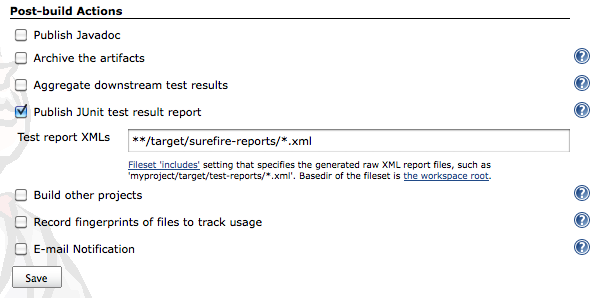
\includegraphics[scale=0.5]{slike/test_xml_path.png}
\end{center}
\caption{Podešavanje putanje za XML izveštaj}
\label{fig:test_xml_path}
\end{figure}

Kada je konfigurisan test izveštaj, Jenkins na početnoj strani projekta prikazuje grafikon na kome se mere za uspešne i neuspešne testove. Kao što se sa slike  \ref{fig:test_project_home} vidi, uspešni su obojeni plavom bojom, dok su neuspešni obojeni crvenom bojom. 

\begin{figure}
\begin{center}
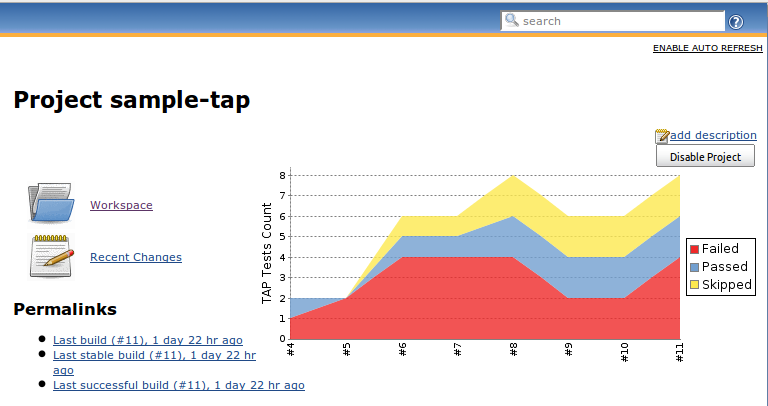
\includegraphics[scale=0.45]{slike/test_project_home.png}
\end{center}
\caption{Početna strana projekta sa izveštajem}
\label{fig:test_project_home}
\end{figure}

U sekciji sa linkovima na početnoj strani možemo videti poslednji build, poslednji stabilni build i poslednji uspešni build. Izborom linka za poslednji build prelazimo na ekran sa detaljima o tom buildu. Na slici \ref{fig:test_last_build} je prikazan ekran sa detaljima. U detaljima Jenkins nam prikazuje koji testovi nisu prosli. Klikom na link neuspešnog testa dobijamo ekran sa detaljima zašto određeni test nije prošao. Ovako se jednostavno fokusiramo na greške i možemo ih brže ispraviti.

\begin{figure}
\begin{center}
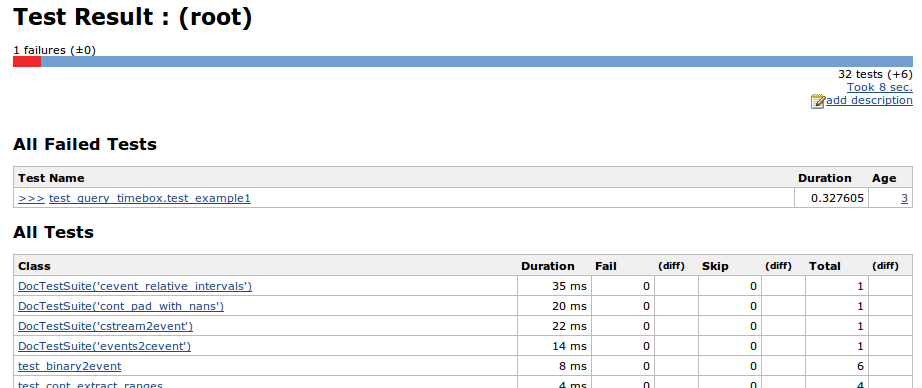
\includegraphics[scale=0.35]{slike/test_last_build.png}
\end{center}
\caption{Poslednji build sa izveštajem o testovima}
\label{fig:test_last_build}
\end{figure}

Testovi jedinica su dizajnirani tako da budu brzi. Na većim projektima testovi mogu da traju i po par sati, a nekada se oni pokreću i više puta dnevno. Spori testovi troše dragoceno vreme programera. Zato je veoma bitno da se testovi pišu tako da budu efikasni. U tu svrhu veoma je poželjno da imamo povratnu informaciju o tome koliko testovi dugo traju, kako bismo mogli da uvidimo problem. Srećom, Jenkins nam pruža lepu vizuelizaciju koliko dugo su se testovi izvršavali za svaki build. Na slici \ref{fig:buildtimetrend} je prikazan grafikon performansi build-ova koji uključuju testove.

\begin{figure}
\begin{center}
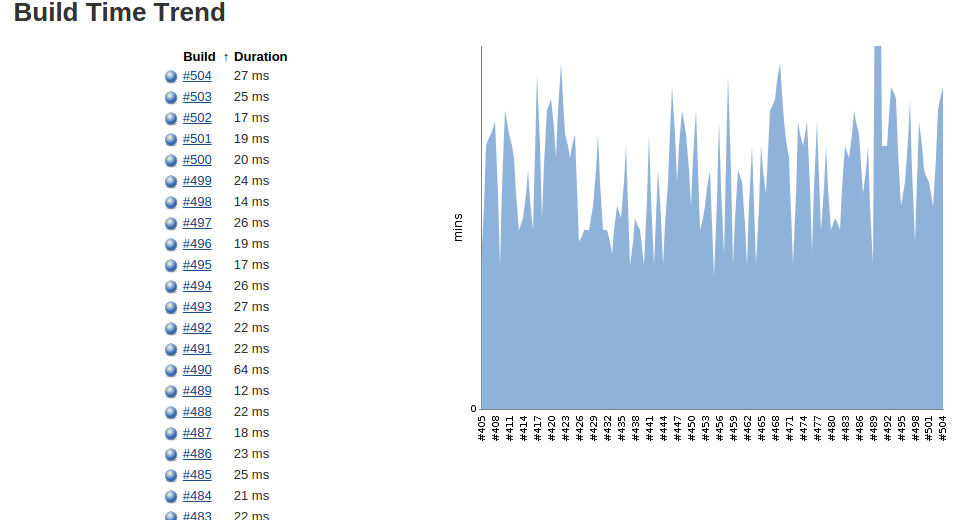
\includegraphics[scale=0.35]{slike/buildtimetrend.png}
\end{center}
\caption{Performanse build-ova}
\label{fig:buildtimetrend}
\end{figure}

\subsection{Pokrivenost k\^oda}
Jedna od metrika koja se ceni u testiranju softvera je \textit{pokrivenost k\^oda}. Iako ona ne daje neku značajnu informaciju o kvalitetu napisanog k\^oda, daje informaciju koliki deo k\^oda je pokriven testovima jedinica. Na primer, ako naši testovi za neku funkcionalnost uvek prolaze kroz \verb|if| granu ali ne i kroz \verb|else| granu.

Standardni alati za testiranje pružaju opcije za pregled pokrivenosti k\^oda u obliku generisanih HTML stranica. Prednost integracije ove metrike u Jenkins je što je možemo pratiti iz build-a u build kroz Jenkins. 

Kao i za većinu funkcionalnosti kod Jenkins sistema, potrebno je instalirati plug-in. Najpoznatiji alat za pokrivenost k\^oda za Javu je Cobertura koji se uključuje u build proces. Izlaz Cobertura alata je XML fajl do kojeg je potrebno da se podesi putanja u Jenkins-u. Tada Jenkins može da iz XML fajla napravi lepe grafikone i lepše prikaže ovu metriku.

Drugi alati, kao na primer PHPUnit, u sebi već imaju ugrađene sisteme za pokrivenost k\^oda. S toga, nije potrebno ništa dodatno podešavati jer plugin-ovi su dovoljno pametni da to prepoznaju i integrišu u Jenkins.

Na slici \ref{fig:test_project_coverage} je prikazano kako izgleda grafikon pokrivenosti k\^oda koji prikazuje Jenkins za ceo projekat. Na sledećoj slici REF možemo pogledati metriku vezanu za određeni paket, dok kad kliknemo na određenu klasu prikazaće nam se k\^od te klase sa obojenom pozadinom koja nam pokazuje koji to delovi k\^oda nisu a koji jesu pokriveni testovima.

\begin{figure}
\begin{center}
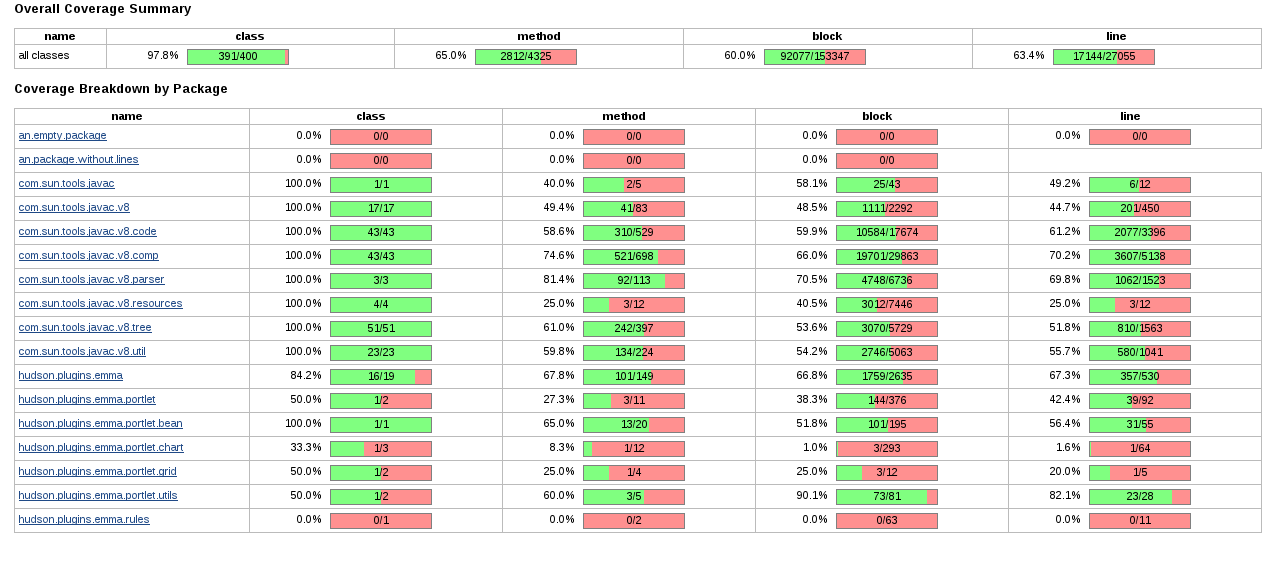
\includegraphics[scale=0.25]{slike/test_project_coverage.png}
\end{center}
\caption{Početna strana projekta sa izveštajem}
\label{fig:test_project_coverage}
\end{figure}




